\chapter{Генетический алгоритм} \label{ParticleSwarmOptimisation}
%\addcontentsline{toc}{chapter}{Метод роения частиц}    % Добавляем его в оглавление, если нет нумерации
\noindent
\emph{Генетический алгоритм} (\emph{Genetic Algorithm}, GA) является одним из самых популярных типов эволюционных алгоритмов, которые — как можно понять из их названия, — используют теорию Дарвина в решении той или иной оптимизационной задачи. Суть алгортима заключается в поиске наилучшего решения по принципу естественного отбора: случайным образом создается поколение, в ходе эволюции которого происходит мутация и скрещевание генов.

\section{Алгоритм, используя real value encoding}
\noindent
Традиционно в качестве решения генетический алгоритм использует бинарное представление (binary encoding). Однако в данной работе будет проиллюстрирован метод именно для реального представления (real value encoding), то есть решение будет представляться в вещественных числах.

Рассмотрим задачу нахождения глобального минимума функции~$F \colon \mathbb{R}^n \to \mathbb{R}$:
\[
	\mathop{\mathrm{argmin}}_{x \in \mathbb{R}^n}f(x),
\]
где каждая особь кодируется вектором $x = (x_1, ..., x_n)$, называемым хромосомой, компоненты которого являются генами.

\begin{figure}[!h]
\centering
\tikzset{every picture/.style={line width=0.75pt}} %set default line width to 0.75pt

\begin{tikzpicture}[x=0.75pt,y=0.75pt,yscale=-1,xscale=1]
%uncomment if require: \path (0,739); %set diagram left start at 0, and has height of 739

%Shape: Rectangle [id:dp8612057014709158]
\draw   (80,71) -- (110.5,71) -- (110.5,100) -- (80,100) -- cycle ;
%Shape: Rectangle [id:dp9416262412972431]
\draw   (110.5,71) -- (141,71) -- (141,100) -- (110.5,100) -- cycle ;
%Shape: Rectangle [id:dp9259667143051737]
\draw   (141,71) -- (171.5,71) -- (171.5,100) -- (141,100) -- cycle ;
%Shape: Rectangle [id:dp4285081026342692]
\draw   (171.5,71) -- (202,71) -- (202,100) -- (171.5,100) -- cycle ;
%Shape: Rectangle [id:dp6066867188861804]
\draw   (202,71) -- (232.5,71) -- (232.5,100) -- (202,100) -- cycle ;
%Curve Lines [id:da8858061911822572]
\draw    (232.5,71) .. controls (289.5,72) and (230.5,126) .. (308.5,126) ;
%Straight Lines [id:da05811670243584288]
\draw    (158.5,45) -- (158.5,68) ;
\draw [shift={(158.5,70)}, rotate = 270] [color={rgb, 255:red, 0; green, 0; blue, 0 }  ][line width=0.75]    (10.93,-3.29) .. controls (6.95,-1.4) and (3.31,-0.3) .. (0,0) .. controls (3.31,0.3) and (6.95,1.4) .. (10.93,3.29)   ;
%Shape: Rectangle [id:dp4349277402828884]
\draw   (81,151) -- (111.5,151) -- (111.5,180) -- (81,180) -- cycle ;
%Shape: Rectangle [id:dp24027028194138378]
\draw   (111.5,151) -- (142,151) -- (142,180) -- (111.5,180) -- cycle ;
%Shape: Rectangle [id:dp0500263413916362]
\draw   (142,151) -- (172.5,151) -- (172.5,180) -- (142,180) -- cycle ;
%Shape: Rectangle [id:dp8133255101181311]
\draw   (172.5,151) -- (203,151) -- (203,180) -- (172.5,180) -- cycle ;
%Shape: Rectangle [id:dp367355050028054]
\draw   (203,151) -- (233.5,151) -- (233.5,180) -- (203,180) -- cycle ;
%Curve Lines [id:da7627402544422663]
\draw    (233.5,180) .. controls (290.5,181) and (230.5,126) .. (308.5,126) ;
%Shape: Circle [id:dp7594178378532763]
\draw   (113.75,165.5) .. controls (113.75,158.32) and (119.57,152.5) .. (126.75,152.5) .. controls (133.93,152.5) and (139.75,158.32) .. (139.75,165.5) .. controls (139.75,172.68) and (133.93,178.5) .. (126.75,178.5) .. controls (119.57,178.5) and (113.75,172.68) .. (113.75,165.5) -- cycle ;
%Straight Lines [id:da7888876982561981]
\draw    (161.5,202) -- (131.49,175.33) ;
\draw [shift={(130,174)}, rotate = 401.63] [color={rgb, 255:red, 0; green, 0; blue, 0 }  ][line width=0.75]    (10.93,-3.29) .. controls (6.95,-1.4) and (3.31,-0.3) .. (0,0) .. controls (3.31,0.3) and (6.95,1.4) .. (10.93,3.29)   ;

% Text Node
\draw (80,122) node [anchor=north west][inner sep=0.75pt]   [align=left] {..............................};
% Text Node
\draw (311,120) node [anchor=north west][inner sep=0.75pt]  [font=\small] [align=left] {Популяция};
% Text Node
\draw (123,30) node [anchor=north west][inner sep=0.75pt]  [font=\small] [align=left] {Хромосома};
% Text Node
\draw (85,78) node [anchor=north west][inner sep=0.75pt]  [font=\small] [align=left] {$\displaystyle x_{11}$};
% Text Node
\draw (146,78) node [anchor=north west][inner sep=0.75pt]  [font=\small] [align=left] {$\displaystyle x_{13}$};
% Text Node
\draw (207,78) node [anchor=north west][inner sep=0.75pt]  [font=\small] [align=left] {$\displaystyle x_{1n}$};
% Text Node
\draw (115.5,78) node [anchor=north west][inner sep=0.75pt]  [font=\small] [align=left] {$\displaystyle x_{12}$};
% Text Node
\draw (179,82) node [anchor=north west][inner sep=0.75pt]   [align=left] {...};
% Text Node
\draw (86,158) node [anchor=north west][inner sep=0.75pt]  [font=\small] [align=left] {$\displaystyle x_{\ell 1}$};
% Text Node
\draw (147,158) node [anchor=north west][inner sep=0.75pt]  [font=\small] [align=left] {$\displaystyle x_{\ell 3}$};
% Text Node
\draw (208,158) node [anchor=north west][inner sep=0.75pt]  [font=\small] [align=left] {$\displaystyle x_{\ell n}$};
% Text Node
\draw (116.5,158) node [anchor=north west][inner sep=0.75pt]  [font=\small] [align=left] {$\displaystyle x_{\ell 2}$};
% Text Node
\draw (180,162) node [anchor=north west][inner sep=0.75pt]   [align=left] {...};
% Text Node
\draw (163.5,205) node [anchor=north west][inner sep=0.75pt]  [font=\small] [align=left] {Ген};
\end{tikzpicture}
\caption{}
\end{figure}

Пусть у нашего поколения или популяции ($P$) есть $\ell$ особей. Тогда поколение в момент времени $t$ примет следующий вид:
\[
	P_t = \{x_{i,t}\}_{i=1}^\ell,
\]
где у кажой хромосомы имеется $n$ генов: $x_{i, t} = (x_{i1,t}, ..., x_{in, t})$


\begin{figure}[!h]
	\centering


	\tikzset{every picture/.style={line width=0.75pt}} %set default line width to 0.75pt

	\begin{tikzpicture}[x=0.75pt,y=0.75pt,yscale=-1,xscale=1]
	%uncomment if require: \path (0,739); %set diagram left start at 0, and has height of 739


	%Rounded Rect [id:dp6834144691063508]
	\draw  [color={rgb, 255:red, 128; green, 128; blue, 128 }  ,draw opacity=1 ][fill={rgb, 255:red, 155; green, 155; blue, 155 }  ,fill opacity=0.06 ] (240.5,57) .. controls (240.5,48.16) and (247.66,41) .. (256.5,41) -- (474.5,41) .. controls (483.34,41) and (490.5,48.16) .. (490.5,57) -- (490.5,105) .. controls (490.5,113.84) and (483.34,121) .. (474.5,121) -- (256.5,121) .. controls (247.66,121) and (240.5,113.84) .. (240.5,105) -- cycle ;
	%Rounded Rect [id:dp6349764616806755]
	\draw   (400.5,316) .. controls (400.5,307.16) and (407.66,300) .. (416.5,300) -- (634.5,300) .. controls (643.34,300) and (650.5,307.16) .. (650.5,316) -- (650.5,364) .. controls (650.5,372.84) and (643.34,380) .. (634.5,380) -- (416.5,380) .. controls (407.66,380) and (400.5,372.84) .. (400.5,364) -- cycle ;
	%Rounded Rect [id:dp3411925739284387]
	\draw   (79.5,316) .. controls (79.5,307.16) and (86.66,300) .. (95.5,300) -- (313.5,300) .. controls (322.34,300) and (329.5,307.16) .. (329.5,316) -- (329.5,364) .. controls (329.5,372.84) and (322.34,380) .. (313.5,380) -- (95.5,380) .. controls (86.66,380) and (79.5,372.84) .. (79.5,364) -- cycle ;
	%Rounded Rect [id:dp15356651288080547]
	\draw  [color={rgb, 255:red, 128; green, 128; blue, 128 }  ,draw opacity=1 ][fill={rgb, 255:red, 155; green, 155; blue, 155 }  ,fill opacity=0.06 ] (241.5,187) .. controls (241.5,178.16) and (248.66,171) .. (257.5,171) -- (475.5,171) .. controls (484.34,171) and (491.5,178.16) .. (491.5,187) -- (491.5,235) .. controls (491.5,243.84) and (484.34,251) .. (475.5,251) -- (257.5,251) .. controls (248.66,251) and (241.5,243.84) .. (241.5,235) -- cycle ;
	%Rounded Rect [id:dp13735168020488797]
	\draw  [color={rgb, 255:red, 128; green, 128; blue, 128 }  ,draw opacity=1 ][fill={rgb, 255:red, 155; green, 155; blue, 155 }  ,fill opacity=0.06 ] (400.5,316) .. controls (400.5,307.16) and (407.66,300) .. (416.5,300) -- (634.5,300) .. controls (643.34,300) and (650.5,307.16) .. (650.5,316) -- (650.5,364) .. controls (650.5,372.84) and (643.34,380) .. (634.5,380) -- (416.5,380) .. controls (407.66,380) and (400.5,372.84) .. (400.5,364) -- cycle ;
	%Rounded Rect [id:dp18159494190384895]
	\draw  [color={rgb, 255:red, 128; green, 128; blue, 128 }  ,draw opacity=1 ][fill={rgb, 255:red, 155; green, 155; blue, 155 }  ,fill opacity=0.06 ] (240.5,446) .. controls (240.5,437.16) and (247.66,430) .. (256.5,430) -- (474.5,430) .. controls (483.34,430) and (490.5,437.16) .. (490.5,446) -- (490.5,494) .. controls (490.5,502.84) and (483.34,510) .. (474.5,510) -- (256.5,510) .. controls (247.66,510) and (240.5,502.84) .. (240.5,494) -- cycle ;
	%Rounded Rect [id:dp23454056652855249]
	\draw  [color={rgb, 255:red, 128; green, 128; blue, 128 }  ,draw opacity=1 ][fill={rgb, 255:red, 155; green, 155; blue, 155 }  ,fill opacity=0.06 ] (79.5,316) .. controls (79.5,307.16) and (86.66,300) .. (95.5,300) -- (313.5,300) .. controls (322.34,300) and (329.5,307.16) .. (329.5,316) -- (329.5,364) .. controls (329.5,372.84) and (322.34,380) .. (313.5,380) -- (95.5,380) .. controls (86.66,380) and (79.5,372.84) .. (79.5,364) -- cycle ;
	%Rounded Rect [id:dp04080350160967616]
	\draw  [color={rgb, 255:red, 128; green, 128; blue, 128 }  ,draw opacity=1 ][fill={rgb, 255:red, 155; green, 155; blue, 155 }  ,fill opacity=0.06 ] (140.38,566.82) .. controls (140.38,563.61) and (142.99,561) .. (146.2,561) -- (324.56,561) .. controls (327.77,561) and (330.38,563.61) .. (330.38,566.82) -- (330.38,584.28) .. controls (330.38,587.49) and (327.77,590.1) .. (324.56,590.1) -- (146.2,590.1) .. controls (142.99,590.1) and (140.38,587.49) .. (140.38,584.28) -- cycle ;
	%Rounded Rect [id:dp20329352519352284]
	\draw  [color={rgb, 255:red, 128; green, 128; blue, 128 }  ,draw opacity=1 ][fill={rgb, 255:red, 155; green, 155; blue, 155 }  ,fill opacity=0.06 ] (400.38,566.82) .. controls (400.38,563.61) and (402.99,561) .. (406.2,561) -- (584.56,561) .. controls (587.77,561) and (590.38,563.61) .. (590.38,566.82) -- (590.38,584.28) .. controls (590.38,587.49) and (587.77,590.1) .. (584.56,590.1) -- (406.2,590.1) .. controls (402.99,590.1) and (400.38,587.49) .. (400.38,584.28) -- cycle ;
	%Straight Lines [id:da8542759790833123]
	\draw [line width=0.75]    (100.5,381) -- (100.01,458) ;
	\draw [shift={(100,460)}, rotate = 270.36] [color={rgb, 255:red, 0; green, 0; blue, 0 }  ][line width=0.75]    (15.3,-6.86) .. controls (9.73,-3.22) and (4.63,-0.93) .. (0,0) .. controls (4.63,0.93) and (9.73,3.22) .. (15.3,6.86)   ;
	%Curve Lines [id:da3464775501690811]
	\draw    (492,210) .. controls (540.51,210) and (529.23,248.22) .. (529.97,298.47) ;
	\draw [shift={(530,300)}, rotate = 268.88] [color={rgb, 255:red, 0; green, 0; blue, 0 }  ][line width=0.75]    (10.93,-4.9) .. controls (6.95,-2.3) and (3.31,-0.67) .. (0,0) .. controls (3.31,0.67) and (6.95,2.3) .. (10.93,4.9)   ;
	%Curve Lines [id:da05243098101616073]
	\draw    (530,381) .. controls (530,430.5) and (537.84,469.22) .. (491.42,469.99) ;
	\draw [shift={(490,470)}, rotate = 360] [color={rgb, 255:red, 0; green, 0; blue, 0 }  ][line width=0.75]    (10.93,-4.9) .. controls (6.95,-2.3) and (3.31,-0.67) .. (0,0) .. controls (3.31,0.67) and (6.95,2.3) .. (10.93,4.9)   ;
	%Curve Lines [id:da3734166178553002]
	\draw    (239,470) .. controls (190.49,470) and (199.81,431.78) .. (200,382.5) ;
	\draw [shift={(200,381)}, rotate = 450] [color={rgb, 255:red, 0; green, 0; blue, 0 }  ][line width=0.75]    (10.93,-4.9) .. controls (6.95,-2.3) and (3.31,-0.67) .. (0,0) .. controls (3.31,0.67) and (6.95,2.3) .. (10.93,4.9)   ;
	%Curve Lines [id:da337716542230607]
	\draw    (199,299) .. controls (199.99,251.48) and (190.2,210.82) .. (239.49,210.01) ;
	\draw [shift={(241,210)}, rotate = 180] [color={rgb, 255:red, 0; green, 0; blue, 0 }  ][line width=0.75]    (10.93,-4.9) .. controls (6.95,-2.3) and (3.31,-0.67) .. (0,0) .. controls (3.31,0.67) and (6.95,2.3) .. (10.93,4.9)   ;
	%Straight Lines [id:da3596375703194834]
	\draw  [dash pattern={on 0.84pt off 2.51pt}]  (359,511) -- (240,557) ;
	%Straight Lines [id:da6375981239192003]
	\draw  [dash pattern={on 0.84pt off 2.51pt}]  (359,511) -- (498,561) ;
	%Straight Lines [id:da4776300035987695]
	\draw [line width=0.75]    (364.5,121) -- (364.98,170) ;
	\draw [shift={(365,172)}, rotate = 269.44] [color={rgb, 255:red, 0; green, 0; blue, 0 }  ][line width=0.75]    (15.3,-6.86) .. controls (9.73,-3.22) and (4.63,-0.93) .. (0,0) .. controls (4.63,0.93) and (9.73,3.22) .. (15.3,6.86)   ;

	% Text Node
	\draw (300,180) node [anchor=north west][inner sep=0.75pt]  [font=\small,rotate=-359.78] [align=left] {\begin{minipage}[lt]{86.87pt}\setlength\topsep{0pt}
	\begin{center}
	{\fontfamily{helvet}\selectfont Расчет функции }\\{\fontfamily{helvet}\selectfont приспособленности}
	\end{center}

	\end{minipage}};
	% Text Node
	\draw (300,50) node [anchor=north west][inner sep=0.75pt]  [font=\small] [align=left] {\begin{minipage}[lt]{93.95696000000001pt}\setlength\topsep{0pt}
	\begin{center}
	{\fontfamily{helvet}\selectfont Создание поколения }\\t = 0
	\end{center}

	\end{minipage}};
	% Text Node
	\draw (500,331.8) node [anchor=north west][inner sep=0.75pt]  [font=\small] [align=left] {Отбор};
	% Text Node
	\draw (190,567.8) node [anchor=north west][inner sep=0.75pt]  [font=\small] [align=left] {Срещивание};
	% Text Node
	\draw (470,567.76) node [anchor=north west][inner sep=0.75pt]  [font=\small] [align=left] {Мутация};
	% Text Node
	\draw (90,333.8) node [anchor=north west][inner sep=0.75pt]  [font=\small] [align=left] {Критерий останова выполнен?};
	% Text Node
	\draw (260,440) node [anchor=north west][inner sep=0.75pt]  [font=\small] [align=left] {\begin{minipage}[lt]{144.88216000000003pt}\setlength\topsep{0pt}
	\begin{center}
	Формирование нового поколения\\t = t + 1
	\end{center}

	\end{minipage}};
	% Text Node
	\draw (165,246.8) node [anchor=north west][inner sep=0.75pt]  [font=\small] [align=left] {Нет};
	% Text Node
	\draw (109.5,404.8) node [anchor=north west][inner sep=0.75pt]  [font=\small] [align=left] {Да};
	% Text Node
	\draw (82.5,463.8) node [anchor=north west][inner sep=0.75pt]  [font=\small] [align=left] {Выход};
	\end{tikzpicture}
	\caption{ --- Генетический алгоритм.}
\end{figure}

Теперь рассмотрим сам алгоритм:

\begin{enumerate}
	\item Генерируем первое поколение особей случайным образом:
	\[
		P_0 = \{x_{1, 0}, ..., x_{\ell, 0} \ | \ (x_{i1, 0}, ..., x_{in, 0}) \in D, \  x_{ij, 0} \sim U(a, b)\},
	\]
	где $D = \{(x_1, ..., x_n) \in \mathbb{R}^n \ | \  a < x_i < b,\ \ a,\ b \in \mathbb{R} \} $~--- заданная область оптимизации (гиперкуб или гиперпрямоугольник).

	\item Оцениваем приспособленность (fitness) текущего поколения.
	Сначала вычисляем значения целевой функции  для каждой особи
	\[
		F_t = \{f(x_{i,t})\}_{i=1}^\ell
	\]

	Воспользуемся таким преобразованием $\sigma$, что все комоненты $F_t$ будут лежать на полуинтервале $(0, 1]$:
	\[
		\sigma(z) = \dfrac{z - F^{worst}}{F^{best} - F^{worst}},
	\]
	где $F^{best}$, $F^{worst}$~--- лучший и худший значения целевой функции в текущем поколении соответственно.


	Тогда получим значения приспособленности особей:
	\[
	F'_t = \{\sigma(f(x_{i, t}))\}_{i=1}^\ell
	\]

	\item  Отбирем $k$ наиболее преспособленных особей для дальнейшего размножения.

	Будем считать, что особь $x'$ более приспособлена, чем особь $x''$, если
	\[
		\sigma(f(x')) > \sigma(f(x''))
	\]

	Ранжируем особи в популяции по значениям их приспособленности в порядке убывания, то есть от самых приспособленных к самым неприспособленным:
	\[
		\sigma(f(x^{(1)}_t)) \geq ... \geq \sigma(f(x^{(k)}_t)) \geq ... \geq \sigma(f(x^{(\ell)}_t))
	\]

	\item Скрещиваем k наиболее приспособленных особей со случайной особью в популяции --- кроме самой лучшей, --- то есть $x^{(1)}_t$. Так мы распространяем <<хорошие>> гены по популяции.

	Под скрещиванием будем иметь в виду операцию создания новой особи, — есле точнее новой хромосомы, — у которой часть генов будет от особи $x$ с вероятностью $\mathbb{P}(z_i = x_i)$, а часть от особи $y$ с вероятностью $\mathbb{P}(z_i = y_i)$.
	\[
		\exists x_t, y_t \in D \colon \Psi(x_t,y_t) = z_{t + 1} = (z_{1,t + 1}, ..., z_{n, t + 1}),
	\]
	где $\Psi$ --- оператор скрещивания особей $x$ и $y$ для получения особи $z$.
\[
z_i
=
\begin{cases}
	x_i, \ \mathbb{P}(z_i = x_i) = \dfrac{\sigma(f(x))}{\sigma(f(x)) + \sigma(f(y))} \\
	\vspace{-5pt} \\
	y_i, \ \mathbb{P}(z_i = y_i) = \dfrac{\sigma(f(y))}{\sigma(f(x)) + \sigma(f(y))}
\end{cases}
\]

Также заметим, что, во-первых, $\mathbb{P}(z_i = x_i) + \mathbb{P}(z_i = y_i) = 1$, а во-вторых,  гены более приспособленной особи чаще присваиваются, нежели случайно выбранной особи. Это объясняется тем, что вероятность получения гена приспособленной особи превышает вероятность  получения гена случайно выбранной особи в большинстве случаев.

\item Некоторых особей в текущей популяции подвергнем мутации. Оператор мутации просто меняет произвольное число генов в хромосоме особи на другие довольно близкие к исходным генам.
\[
	\Upsilon(x_t) = \hat{x}_{t+1},
\]
где $\Upsilon$ --- оператор мутации, а $x$ --- мутируемая особь.

Если ген подвергается мутации, то он принимает следующий вид:
\[
\hat{x}_i
= x_i + \delta_i \in D
\]
	\item Перходим к пункту 2, пока не выполнен критерий останова.

	Примеры критерия останова:
	\begin{enumerate}
		\item достижение заданного количества поколений
		\item точность найденного приближения

на количество поколений (итераций), или на качестве найденного приближения.
	\end{enumerate}
\end{enumerate}

\section{Функция Экли}
\noindent
Функция Экли также как и функция Розенброка используется в качестве оценки производительности оптимизационных алоритмов. Она имеет следующий вид:
 \[
 	f(x_1, ..., x_n)
	=
	20
	+
	e
	-20\exp\left\{-0.2
	\sqrt{\dfrac{1}{n}
	\sum_{i=1}^n \limits x^2_i}
	\right\}
	-
	\exp\left\{
	\dfrac{1}{n}
	\sum_{i=1}^n \limits
	\cos(2\pi x_i)
	\right\}
 \]
 Будем рассматривать трехмерный случай. Тогда глобальный минимум функции Экли достигается в точке $(x, y) = (0, 0)$ со значением целевой функции $f(0, 0) = 0$ (рис. \ref{img:ackley_func}).

 \begin{figure}[h!]
 	\centering
   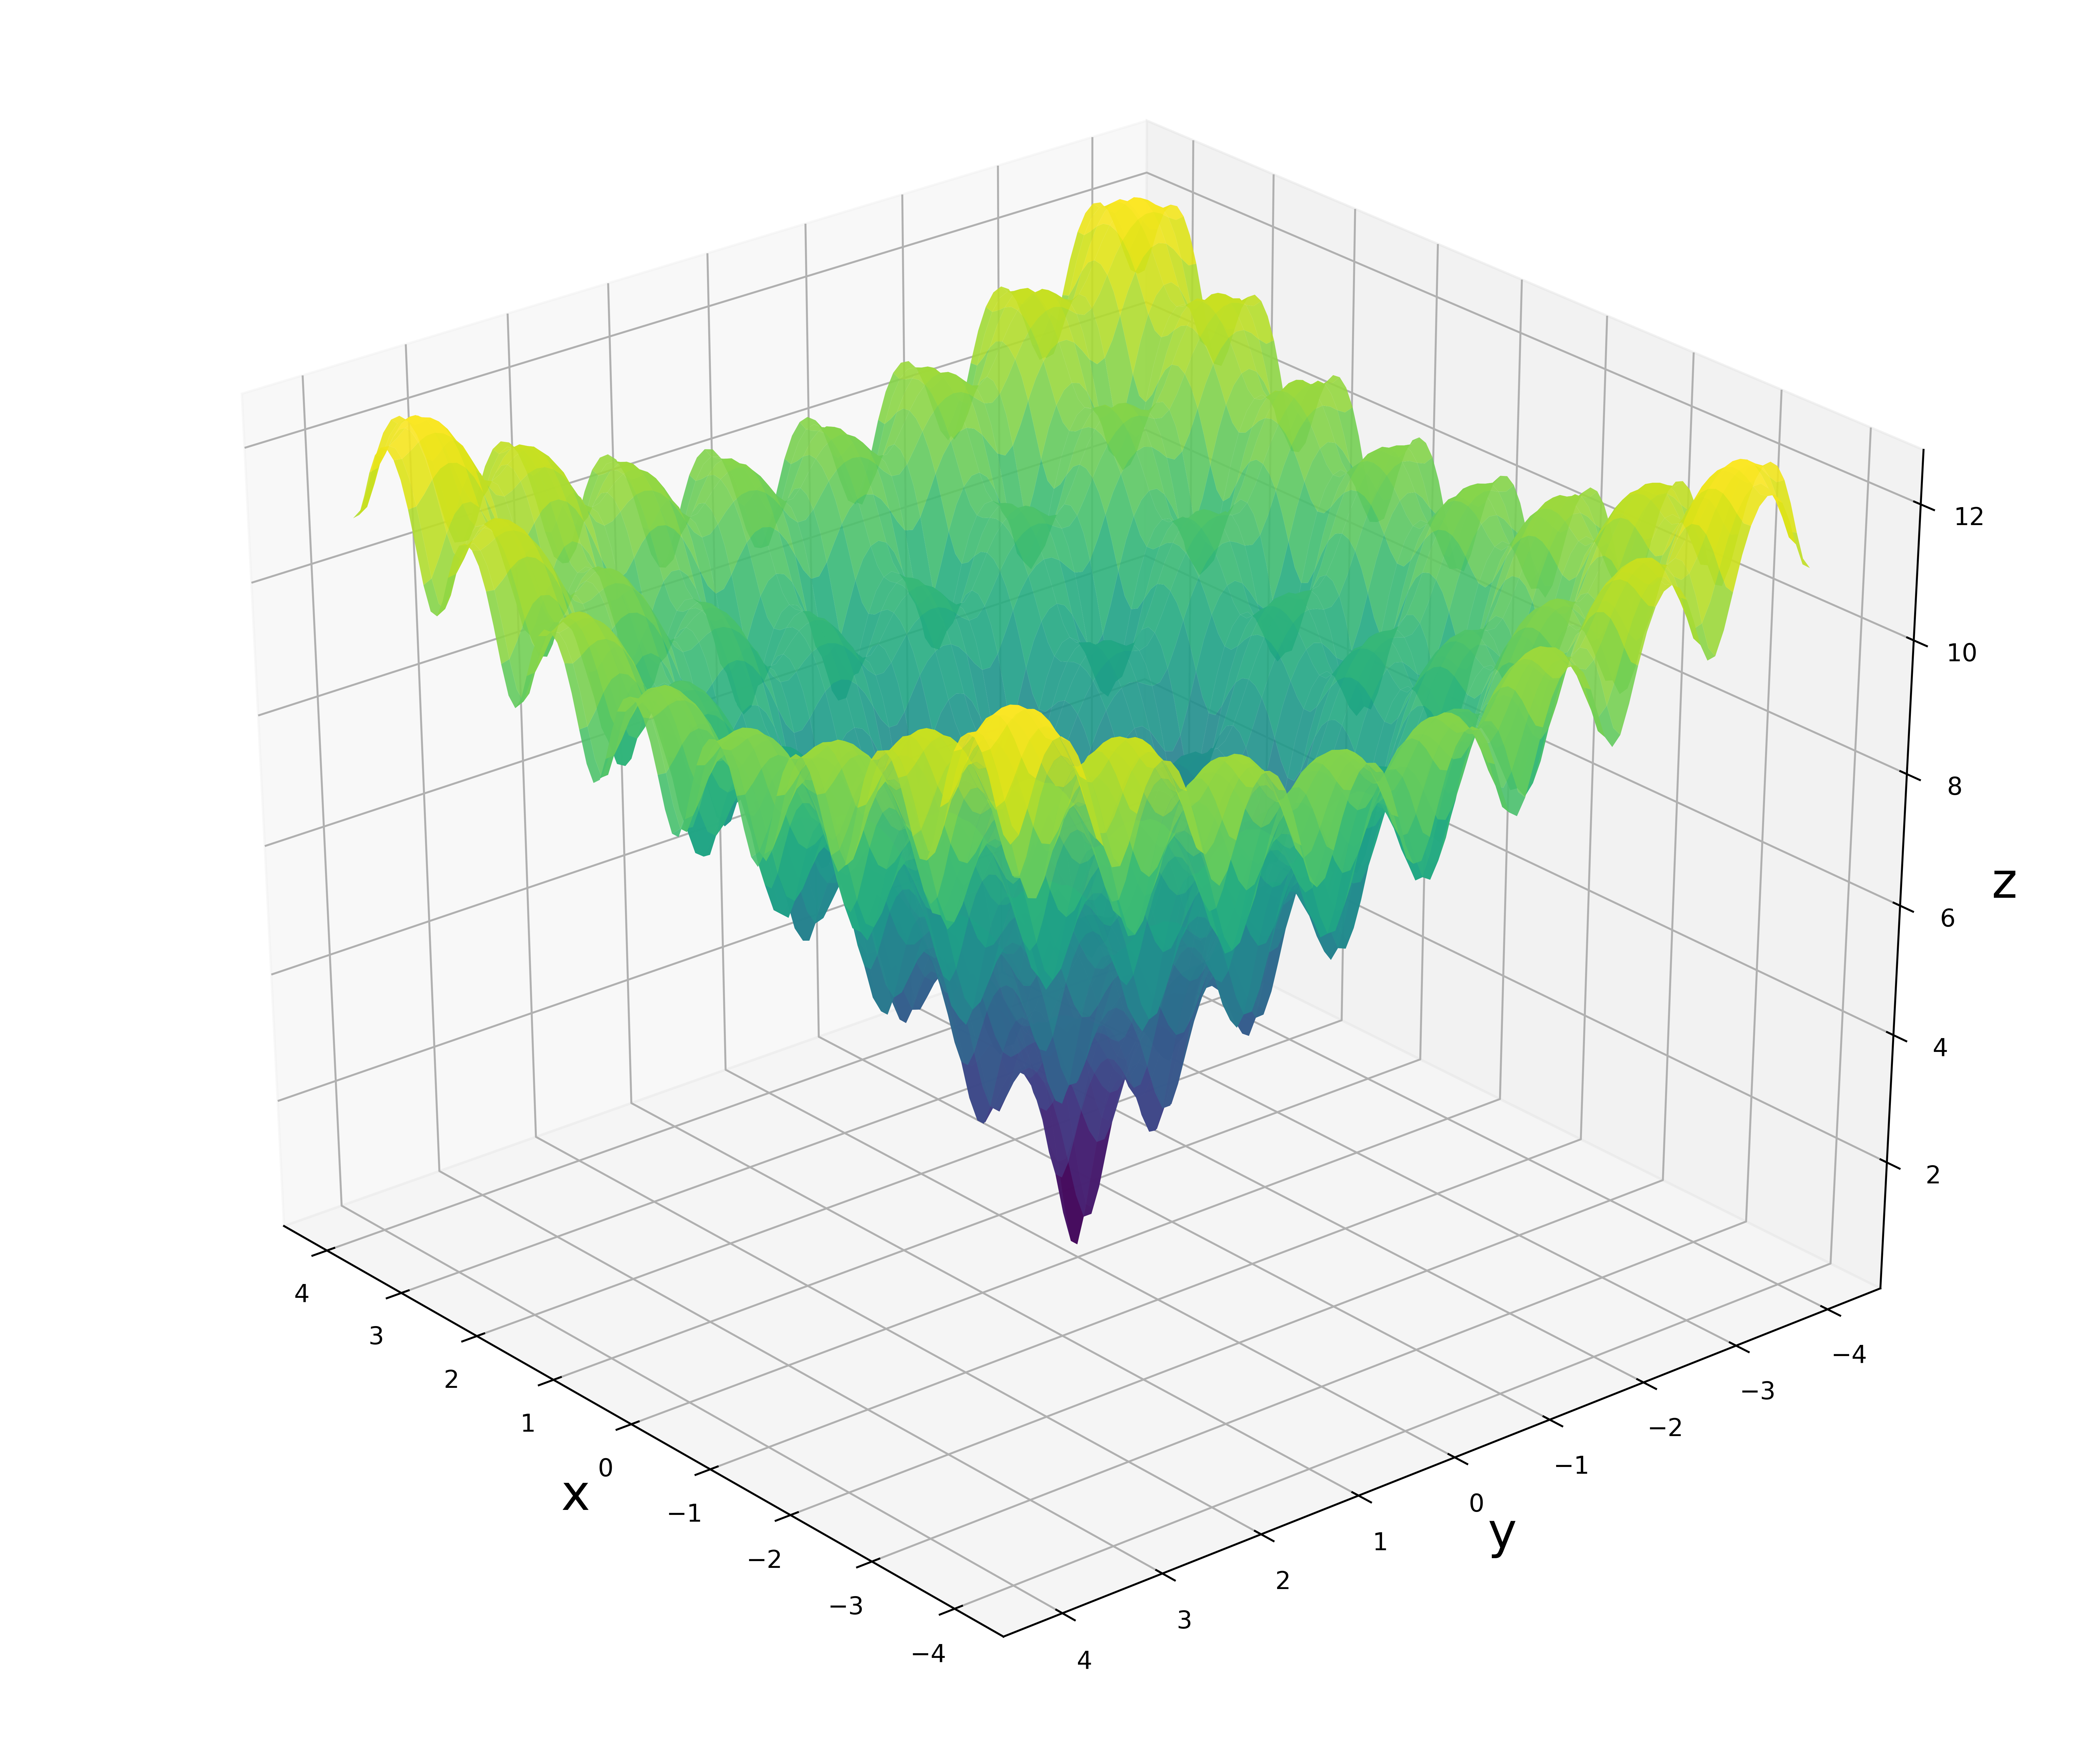
\includegraphics[width=\linewidth]{ackley_func}
   \caption{ --- Функция Экли в трехмерном пространстве.}
   \label{img:ackley_func}
 \end{figure}

\section{Задача коммивояжера}
